% lost-update.tex

\documentclass{standalone}
% newcommands.tex

\newcommand{\enq}{\texttt{enq}}
\newcommand{\deq}{\texttt{deq}}
\newcommand{\pput}{\texttt{PUT}}
\newcommand{\get}{\texttt{GET}}
\newcommand{\vs}{\texttt{vis}}
\newcommand{\so}{\texttt{so}}
\newcommand{\arb}{\texttt{ar}}
\newcommand{\rf}{\texttt{rf}}

% example
\newcommand{\po}[2]{\draw [->, thick] (#1) to node[above] {\Large{\so}} (#2);}
\newcommand{\pva}[2]{\draw [->, thick] (#1) to node[above] {$\Large{\so},\Large{\vs},\Large{\arb}$} (#2);}
\newcommand{\pbva}[2]{\draw [->, thick] (#1) to node[above] {$\Large{\so}$} node[below] {$\Large{\vs},\Large{\arb}$} (#2);}
\newcommand{\pv}[2]{\draw [->, thick] (#1) to node[above] {\Large{\so}} node[below] {\Large{\vs}} (#2);}
\newcommand{\evis}[2]{\draw [->, thick] (#1) to node[above, sloped, near end] {\Large{\vs}} (#2);}
\newcommand{\mvis}[2]{\draw [->, thick] (#1) to node[above, sloped] {\Large{\vs}} (#2);}
\newcommand{\ar}[2]{\draw [->, thick, allow upside down] (#1) to node[above, sloped] {\Large{\arb}} (#2);}
\newcommand{\va}[2]{\draw [->, thick, allow upside down] (#1) to node[above, sloped] {$\Large{\vs},\Large{\arb}$} (#2);}
\newcommand{\vab}[2]{\draw [->, thick, allow upside down] (#1) to node[below, sloped, near end] {$\Large{\vs},\Large{\arb}$} (#2);}
\newcommand{\vae}[2]{\draw [->, thick, allow upside down] (#1) to node[above, sloped, near end] {$\Large{\vs},\Large{\arb}$} (#2);}
\newcommand{\vas}[2]{\draw [->, thick, allow upside down] (#1) to node[sloped, near start, above] {$\Large{\vs},\Large{\arb}$} (#2);}

% serialization
\newcommand{\scc}[2]{\draw [->, very thick] (#1) to (#2);}
\newcommand{\rva}[2]{\draw [->, thick, allow upside down] (#1) to node[above, sloped] {$\Large{\rf},\Large{\vs},\Large{\arb}$} (#2);}
\newcommand{\rvb}[2]{\draw [->, thick, allow upside down] (#1) to node[below, sloped] {$\Large{\rf},\Large{\vs},\Large{\arb}$} (#2);}


\usepackage{tikz}
\usetikzlibrary{shapes, positioning, arrows.meta, decorations.pathmorphing}

\begin{document}
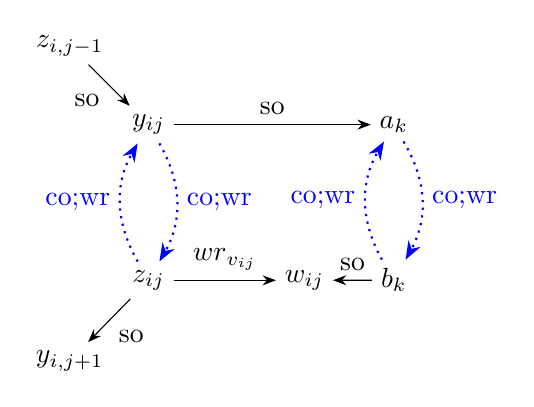
\begin{tikzpicture}[
    wr/.style = {, thick},
    ww/.style = {->, thick, dashed, red},
    rw/.style = {->, thick, dotted, blue},
    txn/.style = {inner sep = 3pt, align = center}]

  \node[txn] (t_yij) {$y_{ij}$};

  \node[txn, right = 2.5cm of t_yij] (t_ak) {$a_k$};
  \node[txn, below = 1.5cm of t_yij] (t_zij) {$z_{ij}$};
  \node[txn, below = 1.5cm of t_ak] (t_bk) {$b_k$};
  \node[txn, right = 1.3cm of t_zij] (t_wij) {$w_{ij}$};

  \draw node at (-1,1) [txn] (t_zijm1) {$z_{i,j-1}$};
  \draw node at (-1,-3) [txn] (t_yijp1) {$y_{i,j+1}$};

  \draw[-Stealth] (t_yij) to node[above]{\red{so}} (t_ak);
  \draw[-Stealth] (t_zij) to node[above]{\red{$\text{wr}_{v_{ij}}$}} (t_wij);
  \draw[-Stealth] (t_bk) to node[above]{\red{so}} (t_wij);
  \draw[-Stealth] (t_zijm1) to node[below left]{\red{so}} (t_yij);
  \draw[-Stealth] (t_zij) to node[below right]{\red{so}} (t_yijp1);

  \draw[-Stealth, dotted, bend left, thick, blue] (t_yij) to node[right]{\red{co;wr}} (t_zij);
  \draw[-Stealth, dotted, bend left, thick, blue] (t_zij) to node[left]{\red{co;wr}} (t_yij);
  \draw[-Stealth, dotted, bend left, thick, blue] (t_ak) to node[right]{\red{co;wr}} (t_bk);
  \draw[-Stealth, dotted, bend left, thick, blue] (t_bk) to node[left]{\red{co;wr}} (t_ak);
\end{tikzpicture}
\end{document}